\documentclass{beamer}
\usetheme{CambridgeUS}
\usefonttheme{serif}
\setbeamertemplate{navigation symbols}{}

\usepackage{ctex}
\usepackage{amsmath,amssymb,amsfonts,bm}
\usepackage{graphicx,subfigure}
\usepackage{adjustbox}
\usepackage{color,xcolor}
\usepackage{tikz}

% 自定义数学公式
\newcommand{\abs}[1]{\left\vert#1\right\vert}
\newcommand{\floor}[1]{\left\lfloor{#1}\right\rfloor}
\newcommand{\ceil}[1]{\left\lceil{#1}\right\rceil}
\newcommand{\sbrace}[1]{\left(#1\right)}
\newcommand{\mbrace}[1]{\left[#1\right]}
\newcommand{\bbrace}[1]{\left\{#1\right\}}
\newcommand{\eval}[2]{\left.{#1}\right|_{#2}}
\newcommand{\conj}[1]{{\rm conj}\sbrace{#1}}
\newcommand{\ALLP}{\mathcal{A}}
\newcommand{\PS}{\mathcal{P}}
\newcommand{\dd}[1]{\mathrm{d}#1}
\newcommand{\ii}[1]{\int\!{#1\dd x}}
\newcommand{\VecNorm}[1]{\left\Vert#1\right\Vert}% 向量模
\newcommand{\spell}[1]{#1}
\newcommand{\up}[1]{^{(#1)}}
\newcommand{\TT}{^\top}% 矩阵转置
\newcommand{\OO}{\ensuremath{\mathbb O}}% n 阶展开多项式余项
\newcommand{\OC}{\ensuremath{\mathcal O}}% 算法复杂度
\newcommand{\lfrac}[2]{#1/#2}
\newcommand{\DIF}[1]{\ensuremath{\frac{\partial}{\partial #1}}}
\newcommand{\DIFF}[2]{\ensuremath{\frac{\partial #1}{\partial #2}}}
\newcommand{\cd}[1]{\,\texttt{#1}\,}
\newcommand{\dbrace}[1]{
  \Bigl\{
    #1
  \Bigr\} 
}
\newcommand{\red}[1]{{\color{red}#1}}

\usepackage{textcomp}
\newcommand{\tpa}{\checkmark}
\newcommand{\tpb}{$-$}
\newcommand{\tpc}{\texttimes}

\newcommand{\Painleve}{Painlev{\'e}}

\title[页脚中部]{大标题}
\author[页脚左侧]{作者}
\date{\today}

\begin{document}
\frame{
    \tikz[overlay,remember picture]\node[opacity=0.1]at (current page.center){
\includegraphics[width=0.7\paperheight]{../paper/sty/ecnu_logo.pdf}};
    \titlepage
}

\section{非线性演化方程的三种波解}
\begin{frame}
\frametitle{非线性演化方程的三种波解}
\begin{enumerate}
\item \Painleve{}展开法得到变换.
\item 简单 Hirota 方法得到孤子解.
\item 共轭参数法得到呼吸子解.
\item 长极限法得到 lump 解.
\item 软件展示 
\end{enumerate}
\end{frame}

\subsection{\Painleve{}展开法}
\begin{frame}
\frametitle{\Painleve{}展开法}
\begin{columns}
\small 
\begin{column}{0.5\textwidth}
理论:
\[
    u=u(x_1,\cdots,x_n,t)
\]
\[
    U(u,u\up{1},u\up{2},u\up{3}\cdots)=0
\]
\[
    u=\sum_{k=1}^m{\frac{u_k}{f^{m-k+1}}}=\frac{u_1}{f^m}+\cdots+\frac{u_m}{f}
\]
\[
    F(f,f\up{1},f\up{2},f\up{3}\cdots)=0
\]
\end{column}
\begin{column}{0.5\textwidth}
例子: (3+1) Jimbo-Miwa 方程
\[
    u_{xxxy}+3u_{xx}u_y+3u_{x}u_{xy}+2u_{ty}-3u_{xz}=0
\]
\[
    u=\frac{2f_x}{f}=2\sbrace{\ln f}_x
\]
\[
\begin{split}
    0&=2\,{f}^{2}f_{{{ txy}}}+{f}^{2}f_{{{ xxxxy}}}-3\,{f}^{2}f_{{{ xxz}}}\\
    &-2\,ff_{{t}}f_{{{ xy}}}-2\,ff_{{{ tx}}}f_{{y}}-2\,ff_{{{ ty}}}f_{{x}}\\
    &-4\,ff_{{x}}f_{{{ xxxy}}}+6\,ff_{{x}}f_{{{ xz}}}+3\,ff_{{{ xx}}}f_{{z}}\\
    &+2\,ff_{{{ xxx}}}f_{{{xy}}}-ff_{{{ xxxx}}}f_{{y}}\\
    &+4\,f_{{t}}f_{{x}}f_{{y}}+6\,{f_{{x}}}^{2}f_{{{ xxy}}}-6\,{f_{{x}}}^{2}f_{{z}}\\
    &-6\,f_{{x}}f_{{{ xx}}}f_{{{ xy}}}+2\,f_{{x}}f_{{{ xxx}}}f_{{y}}
\end{split}
\]
\end{column}
\end{columns}
\end{frame}

\subsection{Hirota 方法与孤子解}
\begin{frame}
\frametitle{Hirota 方法与孤子解}
\begin{columns}
\footnotesize 
\begin{column}{0.5\textwidth}
行波变换:
\[
\begin{split}
    \xi&=p_1\sbrace{x_1+p_2x_2+\cdots+p_nx_n+\omega t} \\ 
    &+p_{n+1}
\end{split}
\]
\[
    \PS\subseteq  \ALLP=\bbrace{1,2,\cdots,n,n+1}
\]
\[
    S(e,k;\PS): \left\{\begin{array}{ll}
        p_i \rightarrow p_{i,k} & i \in \PS, \\ 
        p_i \rightarrow p_i & i \not\in \PS.
    \end{array}\right.
\]
\[
    \xi_i=S(\xi,i,\PS)
\]
理由: 稍后见实验结果.
\end{column}
\begin{column}{0.5\textwidth}
例子:
\[
    \xi=k(x+py+qz+\omega t)+c
\]
\[
    \PS=\bbrace{1,2}
\]
\[
\begin{split}
    \xi_i&=k_i\sbrace{x+p_iy+qz+\frac{3q-k_i^2p_i}{2p_i}t}+c, \\ 
    \xi_j&=k_j\sbrace{x+p_jy+qz+\frac{3q-k_j^2p_j}{2p_j}t}+c.
\end{split} 
\]
\end{column}
\end{columns}
\end{frame}

\begin{frame}
孤子解公式:
\[
\begin{split}
    f_{m-soliton}&=\sum_{\mu=0,1}\exp\sbrace{\sum_{i=1}^m{\mu_i \xi_i}+\sum_{1\le i<j\le m}{\mu_i\mu_jH_{i,j}}} \\ 
    &=\sum_{P\subseteq M}\mbrace{\sbrace{\prod_{\bbrace{i,j}\subseteq P}{h_{i,j}}}\exp\sbrace{\sum_{k\in P}{\xi_k}}} \\ 
\end{split}
\]
\[
    M=\bbrace{1,2,\cdots,m},~~\xi_k=S(\xi,k;\PS)
\]
例子:
\[
\begin{split}
    f_1&=1+\exp\sbrace{\xi_1} \\ 
    f_2&=1+\exp\sbrace{\xi_1}+\exp\sbrace{\xi_2}+h_{1,2}\exp\sbrace{\xi_1+\xi_2} \\ 
    f_3&=1+\exp(\xi_1)+\exp(\xi_2)+\exp(\xi_3)\\
       &+h_{1,2}\exp(\xi_1+\xi_2)+h_{2,3}\exp(\xi_2+\xi_3)+h_{1,3}\exp(\xi_1+\xi_3)\\
       &+h_{1,2}h_{2,3}h_{1,3}\exp(\xi_1+\xi_2+\xi_3)
\end{split}
\]
\end{frame}

\begin{frame} 
\[
\begin{split}
    F(f_1)=0 &\Rightarrow \omega \\ 
    F(f_2)=0 &\Rightarrow h_{i,j} 
\end{split}
\]
\[
\begin{split}
    \omega &= \frac{3q-k^2p}{2p} \\ 
    h_{i,j}&=\frac{(k_ip_j(k_i-k_j)+q)p_i^2-p_ip_j(k_jp_j(k_i-k_j)+2q)+qp_j^2}{(k_ip_j(k_i+k_j)+q)p_i^2+p_ip_j(k_jp_j(k_i+k_j)-2q)+qp_j^2}
\end{split}
\]
\begin{figure}
\centering 
\subfigure[1-孤子解 \label{jm:1-soliton}]{
    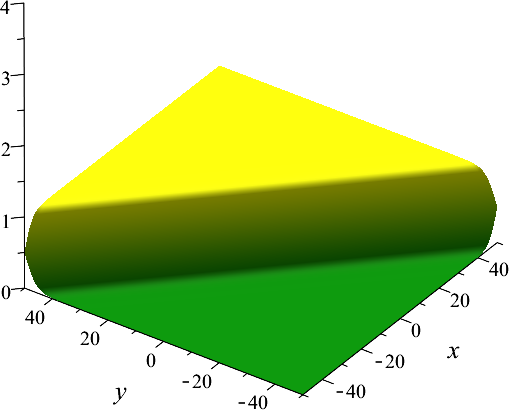
\includegraphics[width=.3\textwidth]{../paper/fig/(3+1)JM-1-soliton.png}    
}
\subfigure[2-孤子解 \label{jm:2-soliton}]{
    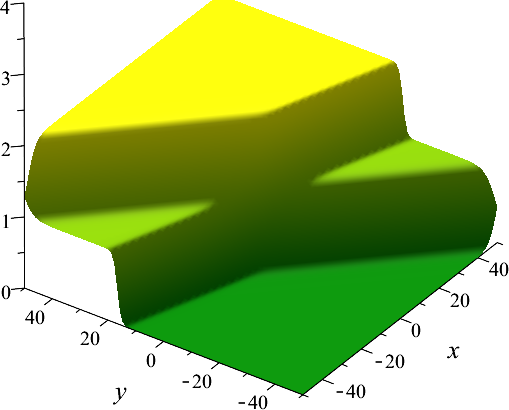
\includegraphics[width=.3\textwidth]{../paper/fig/(3+1)JM-2-soliton.png}
}
\subfigure[3-孤子解 \label{jm:3-soliton}]{
    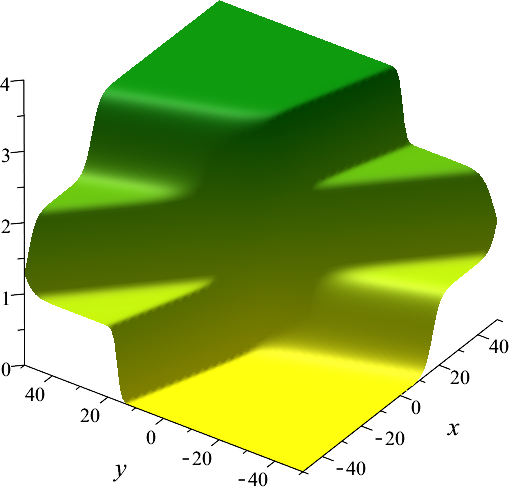
\includegraphics[width=.3\textwidth]{../paper/fig/(3+1)JM-3-soliton.png}
}
\end{figure}
\end{frame}

\subsection{共轭参数法与呼吸子解}
\begin{frame}
\frametitle{共轭参数法与呼吸子解}
\begin{columns}
\begin{column}{0.5\textwidth}
理论:
\[
    f_{m-breather}=\conj{f_{(2m)-soliton}} 
\]
\[
    p_{i,j}=p_{i,j+m}^*,~(j=1,2,\cdots,m)
\]
\[
\begin{split}
    p_{i,j}&=p_{i,j,RE}+I\cdot p_{i,j,IM}, \\ 
    p_{i,j+m}&=p_{i,j,RE}-I\cdot p_{i,j,IM},
\end{split}
\]
\end{column}
\begin{column}{0.5\textwidth}
例子: $m=1,\PS=\bbrace{1,2}$,\\$\xi=k(x+py+qz+\omega t)+c$.
\[
\begin{split}
    k_1&=k_{1,RE}+I\cdot k_{1,IM} \\ 
    k_2&=k_{1,RE}-I\cdot k_{1,IM} \\
    p_1&=p_{1,RE}-I\cdot p_{1,IM} \\
    p_2&=p_{1,RE}+I\cdot p_{1,IM} \\ 
\end{split} 
\]
\end{column}
\end{columns}
\end{frame}

\begin{frame}
\begin{figure}
\setcounter{subfigure}{0}
\subfigure[1-呼吸子解 \label{jm:1-breather}]{
    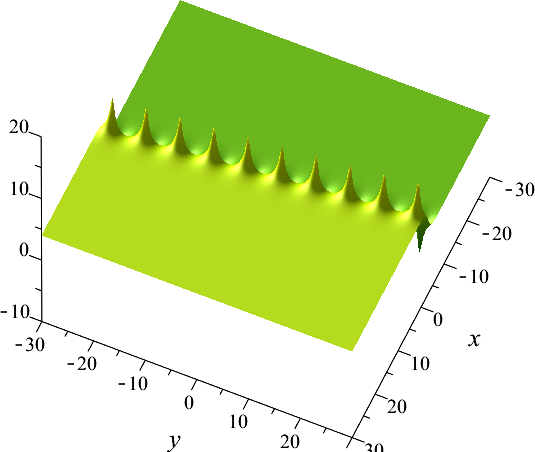
\includegraphics[width=.3\textwidth]{../paper/fig/(3+1)JM-1-breather.png}
}
\subfigure[2-呼吸子解 \label{jm:2-breather}]{
    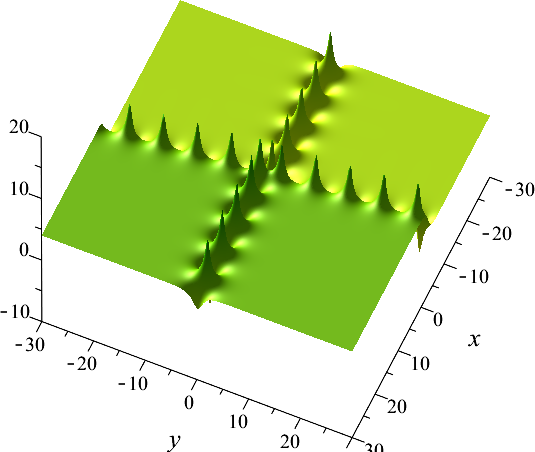
\includegraphics[width=.3\textwidth]{../paper/fig/(3+1)JM-2-breather.png}
}
\subfigure[3-呼吸子解 \label{jm:3-breather}]{
    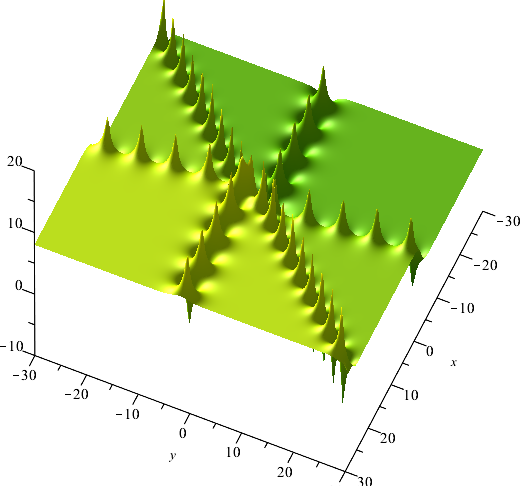
\includegraphics[width=.3\textwidth]{../paper/fig/(3+1)JM-3-breather.png}
}
\subfigure[周期波解 \label{jm:1-periodic}]{
    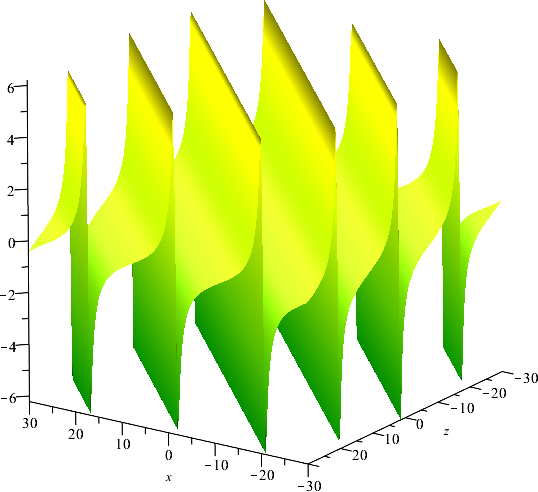
\includegraphics[width=.3\textwidth]{../paper/fig/(3+1)JM-1-periodic.png}
}
\subfigure[孤子-呼吸子相互作用解 \label{jm:soliton-breather}]{
    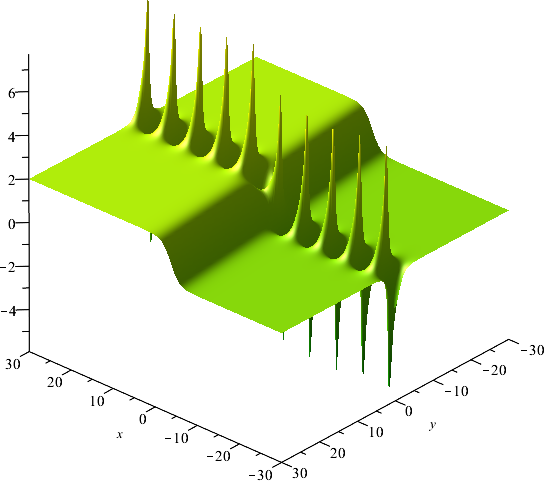
\includegraphics[width=.3\textwidth]{../paper/fig/(3+1)JM-soliton-breather.png}
}
\end{figure}
\end{frame}

\subsection{长极限法与 lump 解}
\begin{frame}{长极限法与 lump 解}
首先, 令
\begin{equation}
\begin{split}
    \xi_i&=k_i\sbrace{x_1+p_ix_2+\cdots+r_ix_n+\omega t}+\xi_i^{(0)},\\
    \eta_i&=\xi_i-\xi_i^{(0)}.
\end{split}
\end{equation}
长极限法的关键在于当$k_i,k_j\rightarrow 0$时, 找到这样两个展开:
\begin{equation}
\begin{split}
    \exp(\eta_i)&=1+k_i \theta_i+o(k_i), \\ 
    h_{i,j}&=1+k_ik_jb_{i,j}+o(k_i^2+k_j^2),
\end{split} \label{lump-expansion}
\end{equation}
其中$o(f)$是Peano余项, 满足$\lim_{f\rightarrow 0}[o(f)/f]=0$.
\end{frame}

\begin{frame}
取$\exp\sbrace{\xi_i^{(0)}}=-1$, 并将上述展开代入到($2m$)-孤子解的生成公式中, 可以得到$m$-lump解. 例如对于一个2-孤子解, 忽略余项后我们有
\begin{equation*}
\begin{split}
\Theta_1&=1+\exp(\xi_1)+\exp(\xi_2)+h_{12}\exp(\xi_1+\xi_2) \\ 
&= 1+\exp(\xi_1)+\exp(\xi_2)+(1+k_1k_2b_{12})\exp(\xi_1+\xi_2) \\ 
&=(1+\exp(\xi_1))(1+\exp(\xi_2))+k_1k_2b_{12}\exp(\eta_1+\eta_2) \\ 
&=(1-(1+k_1\theta_1))(1-(1+k_2\theta_2))+k_1k_2b_{12} \\
&=k_1k_2(\theta_1\theta_2+b_{12}).
\end{split}
\end{equation*}
因为$k_1k_2$是一个能够被TPE消除的常数因子, 所以1-lump解的生成公式为
\begin{equation*}
    \Theta_1=\theta_1\theta_2+b_{12}.
\end{equation*}
\end{frame}
\begin{frame}
推广后可得最终的生成公式为:
\[
    f_{m-lump}=\conj{\Theta_m}
\]
\[
\begin{split}
    \Theta_m&=\prod_{k=1}^{2m}\theta_k+\frac{1}{2}\sum_{i,j}{b_{i,j}}\prod_{J\neq i,j}{\theta_J}+\frac{1}{2! 2^2}\sum_{i,j,k,l}{b_{i,j}b_{k,l}}\prod_{J\neq i,j,k,l}{\theta_{J}}+\cdots \\
    &+\frac{1}{s!2^s}\sum_{i,j,\cdots,u,v}\underbrace{{b_{i,j}b_{k,l}\cdots b_{u,v}}}_{s}\prod_{J\neq i,j,\cdots, u,v}{\theta_J}+\cdots 
\end{split}
\]
例子:
\[
\begin{split}
\Theta_1&=\theta_{1}\theta_{2}+b_{12} \\
\Theta_2&=\theta_{1}\theta_{2}\theta_{3}\theta_{4}+b_{12}\theta_{3}\theta_{4}+b_{13}\theta_{2}\theta_{4}+b_{14}\theta_{2}\theta_{3}+b_{23}\theta_{1}\theta_{4}\\
&+b_{24}\theta_{1}\theta_{3}+b_{34}\theta_{1}\theta_{2}+b_{12}b_{34}+b_{13}b_{34}+b_{14}b_{23}
\end{split}
\]
\end{frame}

\begin{frame}
重写生成公式
\[
    f_{m-lump}=\sum_{l=0}^m\sum_{s\in L(l)}\sbrace{\prod_{k=1}^l{b_{s_{2k-1},s_{2k}}}\prod_{p\not\in s}{\theta_p}}
\]
\[
    L(l)=\bbrace{\sbrace{s_1, s_2, \cdots ,s_{2l}}\left|s_{2k}>s_{2k-1},s_{2k+1}>s_{2k-1},s_k\in \bbrace{1,\cdots,2l}\right.}
\]
\begin{itemize}
\item $s_{2k}>s_{2k-1}$ 保证了$b_{i,j}=b_{j,i}$的等价情况只出现一次. 
\item $s_{2k+1}>s_{2k-1}$ 保证了$b_{i,j}$的全排列只出现一次.
\end{itemize}
\end{frame}

\begin{frame}
\small
\[
\renewcommand{\arraystretch}{0.8} 
\begin{array}{l}
\Theta_3=\theta_{{1}}\theta_{{2}}\theta_{{3}}\theta_{{4}}\theta_{{5}}\theta_{{6}}
+b_{{12}}\theta_{{3}}\theta_{{4}}\theta_{{5}}\theta_{{6}}
+b_{{13}}\theta_{{2}}\theta_{{4}}\theta_{{5}}\theta_{{6}}
+b_{{14}}\theta_{{2}}\theta_{{3}}\theta_{{5}}\theta_{{6}}\\
+b_{{15}}\theta_{{2}}\theta_{{3}}\theta_{{4}}\theta_{{6}}
+b_{{16}}\theta_{{2}}\theta_{{3}}\theta_{{4}}\theta_{{5}}
+b_{{23}}\theta_{{1}}\theta_{{4}}\theta_{{5}}\theta_{{6}}
+b_{{24}}\theta_{{1}}\theta_{{3}}\theta_{{5}}\theta_{{6}}\\
+b_{{25}}\theta_{{1}}\theta_{{3}}\theta_{{4}}\theta_{{6}}
+b_{{26}}\theta_{{1}}\theta_{{3}}\theta_{{4}}\theta_{{5}}
+b_{{34}}\theta_{{1}}\theta_{{2}}\theta_{{5}}\theta_{{6}}
+b_{{35}}\theta_{{1}}\theta_{{2}}\theta_{{4}}\theta_{{6}}\\
+b_{{36}}\theta_{{1}}\theta_{{2}}\theta_{{4}}\theta_{{5}}
+b_{{45}}\theta_{{1}}\theta_{{2}}\theta_{{3}}\theta_{{6}}
+b_{{46}}\theta_{{1}}\theta_{{2}}\theta_{{3}}\theta_{{5}}
+b_{{56}}\theta_{{1}}\theta_{{2}}\theta_{{3}}\theta_{{4}}\\
+b_{{12}}b_{{34}}\theta_{{5}}\theta_{{6}}
+b_{{12}}b_{{35}}\theta_{{4}}\theta_{{6}}
+b_{{12}}b_{{36}}\theta_{{4}}\theta_{{5}}
+b_{{12}}b_{{45}}\theta_{{3}}\theta_{{6}}
+b_{{12}}b_{{46}}\theta_{{3}}\theta_{{5}}\\
+b_{{12}}b_{{56}}\theta_{{3}}\theta_{{4}}
+b_{{13}}b_{{24}}\theta_{{5}}\theta_{{6}}
+b_{{13}}b_{{25}}\theta_{{4}}\theta_{{6}}
+b_{{13}}b_{{26}}\theta_{{4}}\theta_{{5}}
+b_{{13}}b_{{45}}\theta_{{2}}\theta_{{6}}\\
+b_{{13}}b_{{46}}\theta_{{2}}\theta_{{5}}
+b_{{13}}b_{{56}}\theta_{{2}}\theta_{{4}}
+b_{{14}}b_{{23}}\theta_{{5}}\theta_{{6}}
+b_{{14}}b_{{25}}\theta_{{3}}\theta_{{6}}
+b_{{14}}b_{{26}}\theta_{{3}}\theta_{{5}}\\
+b_{{14}}b_{{35}}\theta_{{2}}\theta_{{6}}
+b_{{14}}b_{{36}}\theta_{{2}}\theta_{{5}}
+b_{{14}}b_{{56}}\theta_{{2}}\theta_{{3}}
+b_{{15}}b_{{23}}\theta_{{4}}\theta_{{6}}
+b_{{15}}b_{{24}}\theta_{{3}}\theta_{{6}}\\
+b_{{15}}b_{{26}}\theta_{{3}}\theta_{{4}}
+b_{{15}}b_{{34}}\theta_{{2}}\theta_{{6}}
+b_{{15}}b_{{36}}\theta_{{2}}\theta_{{4}}
+b_{{15}}b_{{46}}\theta_{{2}}\theta_{{3}}
+b_{{16}}b_{{23}}\theta_{{4}}\theta_{{5}}\\
+b_{{16}}b_{{24}}\theta_{{3}}\theta_{{5}}
+b_{{16}}b_{{25}}\theta_{{3}}\theta_{{4}}
+b_{{16}}b_{{34}}\theta_{{2}}\theta_{{5}}
+b_{{16}}b_{{35}}\theta_{{2}}\theta_{{4}}
+b_{{16}}b_{{45}}\theta_{{2}}\theta_{{3}}\\
+b_{{23}}b_{{45}}\theta_{{1}}\theta_{{6}}
+b_{{23}}b_{{46}}\theta_{{1}}\theta_{{5}}
+b_{{23}}b_{{56}}\theta_{{1}}\theta_{{4}}
+b_{{24}}b_{{35}}\theta_{{1}}\theta_{{6}}
+b_{{24}}b_{{36}}\theta_{{1}}\theta_{{5}}\\
+b_{{24}}b_{{56}}\theta_{{1}}\theta_{{3}}
+b_{{25}}b_{{34}}\theta_{{1}}\theta_{{6}}
+b_{{25}}b_{{36}}\theta_{{1}}\theta_{{4}}
+b_{{25}}b_{{46}}\theta_{{1}}\theta_{{3}}
+b_{{26}}b_{{34}}\theta_{{1}}\theta_{{5}}\\
+b_{{26}}b_{{35}}\theta_{{1}}\theta_{{4}}
+b_{{26}}b_{{45}}\theta_{{1}}\theta_{{3}}
+b_{{34}}b_{{56}}\theta_{{1}}\theta_{{2}}
+b_{{35}}b_{{46}}\theta_{{1}}\theta_{{2}}
+b_{{36}}b_{{45}}\theta_{{1}}\theta_{{2}}\\
+b_{{12}}b_{{34}}b_{{56}}
+b_{{12}}b_{{35}}b_{{46}}
+b_{{12}}b_{{36}}b_{{45}}
+b_{{13}}b_{{24}}b_{{56}}
+b_{{13}}b_{{25}}b_{{46}}
+b_{{13}}b_{{26}}b_{{45}}\\
+b_{{14}}b_{{23}}b_{{56}}
+b_{{14}}b_{{25}}b_{{36}}
+b_{{14}}b_{{26}}b_{{35}}
+b_{{15}}b_{{23}}b_{{46}}
+b_{{15}}b_{{24}}b_{{36}}
+b_{{15}}b_{{26}}b_{{34}}\\
+b_{{16}}b_{{23}}b_{{45}}
+b_{{16}}b_{{24}}b_{{35}}
+b_{{16}}b_{{25}}b_{{34}} .
\end{array}
\]
\end{frame}

\begin{frame}{推导关键参数}
将$\eta$看作是一个关于$k$的函数, 我们有一维泰勒展开  
\begin{equation*}
\begin{split}
\exp(\eta(k))&=\exp(\eta(0))+\eta'(0)\exp(\eta(0))k+o(k)\\ 
&=1+\eta'(0)k+o(k). 
\end{split}
\end{equation*}
从而, 
\begin{equation*}
\theta=\eval{\frac{\partial \eta}{\partial k}}{k=0}=\eval{\frac{\partial \xi}{\partial k}}{k=0}.
\end{equation*}
\end{frame}

\begin{frame}
令$h_{i,j}=h(k_i,k_j)$, 根据对称性我们有$h(x,y)=h(y,x)$. 此外, 取$k_2=0$可以将2-孤子解退化为1-孤子解, 所以$h(k_1,0)=1$. 根据对称性, 我们有$h(0,k_2)=1$. 从而, $h(0,0)=1$, 且
\begin{equation*}
    h_x(0,0)=\eval{\frac{\partial}{\partial x}h(x,0)}{x=0}=0.
\end{equation*}
类似地, 我们有$h_y(0,0)=h_{xx}(0,0)=h_{yy}(0,0)=0$. 因此, $h(x,y)$在$(0,0)$点的二维泰勒展开为 
\begin{equation*}
\begin{split}
h(x,y)&=h(0,0)+h_x(0,0)x+h_y(0,0)y \\ 
&+\frac{1}{2}\mbrace{h_{xx}(0,0)x^2+2h_{xy}(0,0)xy+h_{yy}(0,0)y^2}+o(x^2+y^2) \\ 
&=1+h_{xy}(0,0)xy+o(x^2+y^2).
\end{split}
\end{equation*}
从而, 我们得到
\begin{equation*}
    b_{i,j}=\eval{\frac{\partial^2}{\partial k_i\partial k_j}h_{i,j}}{k_i=0,k_j=0}.
\end{equation*}
\end{frame}

\begin{frame}{关键参数结果}
\begin{columns}
\begin{column}{0.5\textwidth}
关键参数:
\[
\begin{split}
    \theta &= \eval{\frac{\partial \xi}{\partial p_1}}{p_1=0}, \\
    b_{i,j}&= \eval{\frac{\partial^2}{\partial p_{1,i}\partial p_{1,j}}h_{i,j}}{p_{1,i}=0,p_{1,j}=0}.
\end{split}
\]
\end{column}
\begin{column}{0.5\textwidth}
例子:
\[
\begin{split}
    &\theta=\frac{2p^2y+(2qz+2x)p+3qt}{2p}, \\ 
    &b_{i,j}=-\frac{2p_ip_j(p_i+p_j)}{q(p_i-p_j)^2}.
\end{split}
\]
\end{column}
\end{columns}
\end{frame}

\begin{frame}
\begin{figure}
\setcounter{subfigure}{0}
\centering 
\subfigure[1-lump解 \label{jm:1-lump}]{
    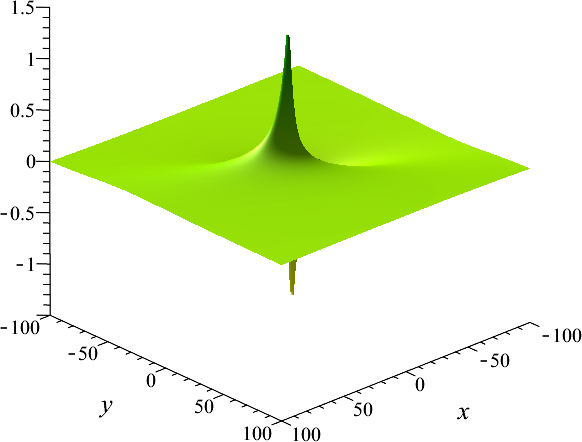
\includegraphics[width=.3\textwidth]{../paper/fig/(3+1)JM-1-lump.png}
}
\subfigure[2-lump解 \label{jm:2-lump}]{
    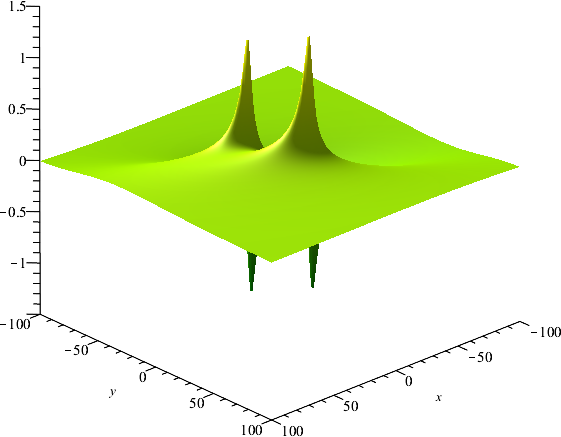
\includegraphics[width=.3\textwidth]{../paper/fig/(3+1)JM-2-lump.png}
}
\subfigure[3-lump解 \label{jm:3-lump}]{
    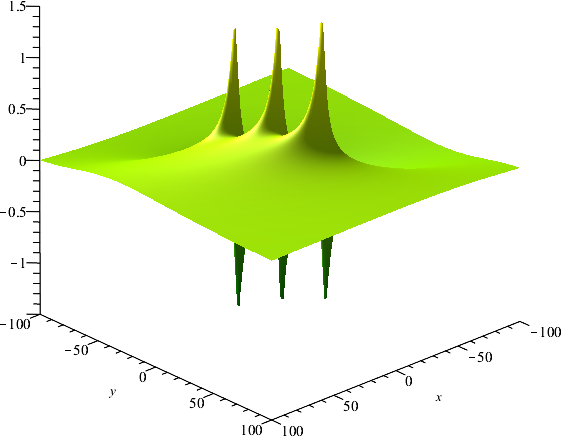
\includegraphics[width=.3\textwidth]{../paper/fig/(3+1)JM-3-lump.png}
}
\subfigure[1-line rogue 解 \label{jm:1-rogue}]{
    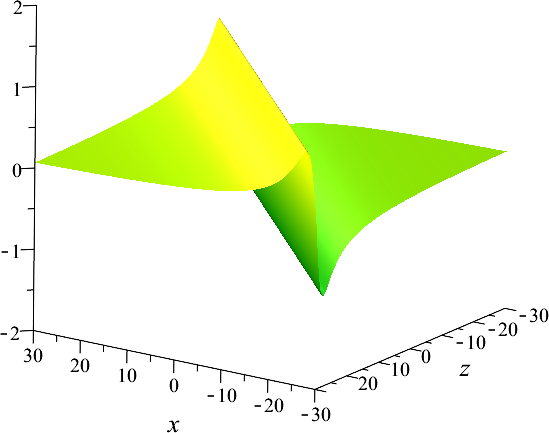
\includegraphics[width=.3\textwidth]{../paper/fig/(3+1)JM-1-rogue.png}
}
\subfigure[2-line rogue 解 \label{jm:2-rogue}]{
    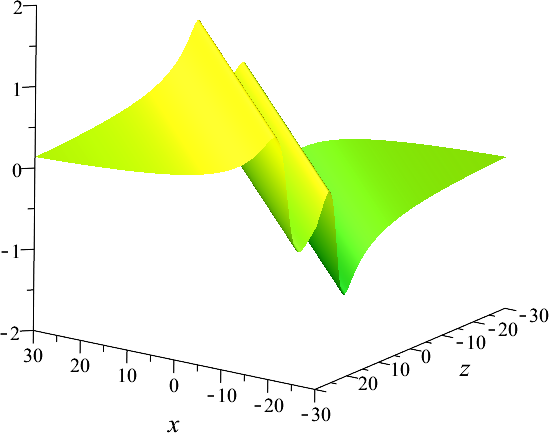
\includegraphics[width=.3\textwidth]{../paper/fig/(3+1)JM-2-rogue.png}
}
\end{figure}
\end{frame}

\subsection{实验与分析}
\begin{frame}
\frametitle{实验与分析}
\begin{columns}
\begin{column}{0.65\textwidth}
\begin{table}
\centering
\small 
\begin{tabular}{lcccc}
\hline
\multicolumn{1}{c}{方程名} & 1 & 12 & 13 & 123 \\ 
\hline
(1+1)KdV & \tpa\tpb & & & \\
(2+1)BKP-T & \tpa\tpb & \tpa\tpa & & \\
(2+1)KP &\tpa\tpb &\tpa\tpa & & \\
(2+1)SK &\tpa\tpb &\tpa\tpa & & \\
(4+1)Fokas-T-2 &\tpa\tpb &\tpa\tpa & & \\
(2+1)CBS & \tpa\tpb & \tpa\tpb & & \\
(2+1)CBS-G & \tpa\tpb & \tpc\tpc & & \\
(3+1)BKP &\tpa\tpb &\tpa\tpa &\tpa\tpa &\tpc\tpc \\
(3+1)KP &\tpa\tpb &\tpa\tpa &\tpa\tpa &\tpc\tpc \\
(3+1)JM &\tpa\tpb &\tpa\tpa &\tpa\tpb &\tpc\tpc \\
(3+1)NEE-T &\tpa\tpb &\tpa\tpa &\tpa\tpb &\tpc\tpc \\
(3+1)YTSF &\tpa\tpb &\tpa\tpa &\tpa\tpb &\tpb\,\tpb \\
(3+1)CBS &\tpa\tpb &\tpa\tpb &\tpa\tpb &\tpa\tpb \\
(4+1)Fokas-T &\tpa\tpb &\tpa\tpb &\tpa\tpb &\tpc\tpc \\
\hline
\end{tabular}
\end{table}
\end{column}
\begin{column}{0.35\textwidth}
\begin{itemize}
\item `\tpa{}' 表示能够满足原方程.
\item `\tpb{}' 表示有解不能得到解.
\item `\tpc{}' 表示有解但不满足原方程.
\item 第一个对应3孤子解, 第二个对应2 lump解.
\end{itemize}
\end{column}
\end{columns}
\end{frame}

\begin{frame}
实验结果:
\begin{itemize}
\item $\PS=\bbrace{1}$, 所有方程都有3-孤子解. 
\item $\PS=\ALLP$, 除了两个CBS方程, 所有(2+1)维的方程都有lump解. 
\item $\PS=\ALLP$, (3+1)YTSF方程没有孤子解, 所以不能先取$\PS=\ALLP$, 再取特殊值使得$\PS\subsetneq \ALLP$. 
\item 大部分(3+1)维方程在$\PS=\bbrace{1,2}$或$\PS=\bbrace{1,3}$是才有孤子解和lump解.
\item 孤子解成立是lump解成立的必要条件. 
\end{itemize}
\end{frame}

\subsection{软件展示}
\begin{frame}{软件展示}
\href{run:D:/Desktop/YjtMapleLib/build/LypReport/TwSolver.mw}{TwSolver.mw}
\begin{itemize}
\item (3+1)JM 方程, 整体流程和绘图结果展示.
\item (2+1)BKP 方程, 积分预处理和\Painleve{}展开结果的选择, 以及不同的绘图方式展示.
\item (4+1)Fokas 方程, 高维方程降维求解的例子.
\end{itemize}
\end{frame}

\section{分组并行求解算法及其应用}
\begin{frame}
\frametitle{分组并行求解算法及其应用}
\begin{enumerate}
\item PGSolve: 分组并行算法
\item NS1L: 求$n$-孤子-1 lump相互作用解的软件包
\item PGSolve 的求解效率
\item 软件展示 
\end{enumerate}
\end{frame}

\subsection{PGSolve: 分组并行求解算法}
\begin{frame}
\frametitle{PGSolve: 分组并行求解算法}
\begin{figure}
\centering
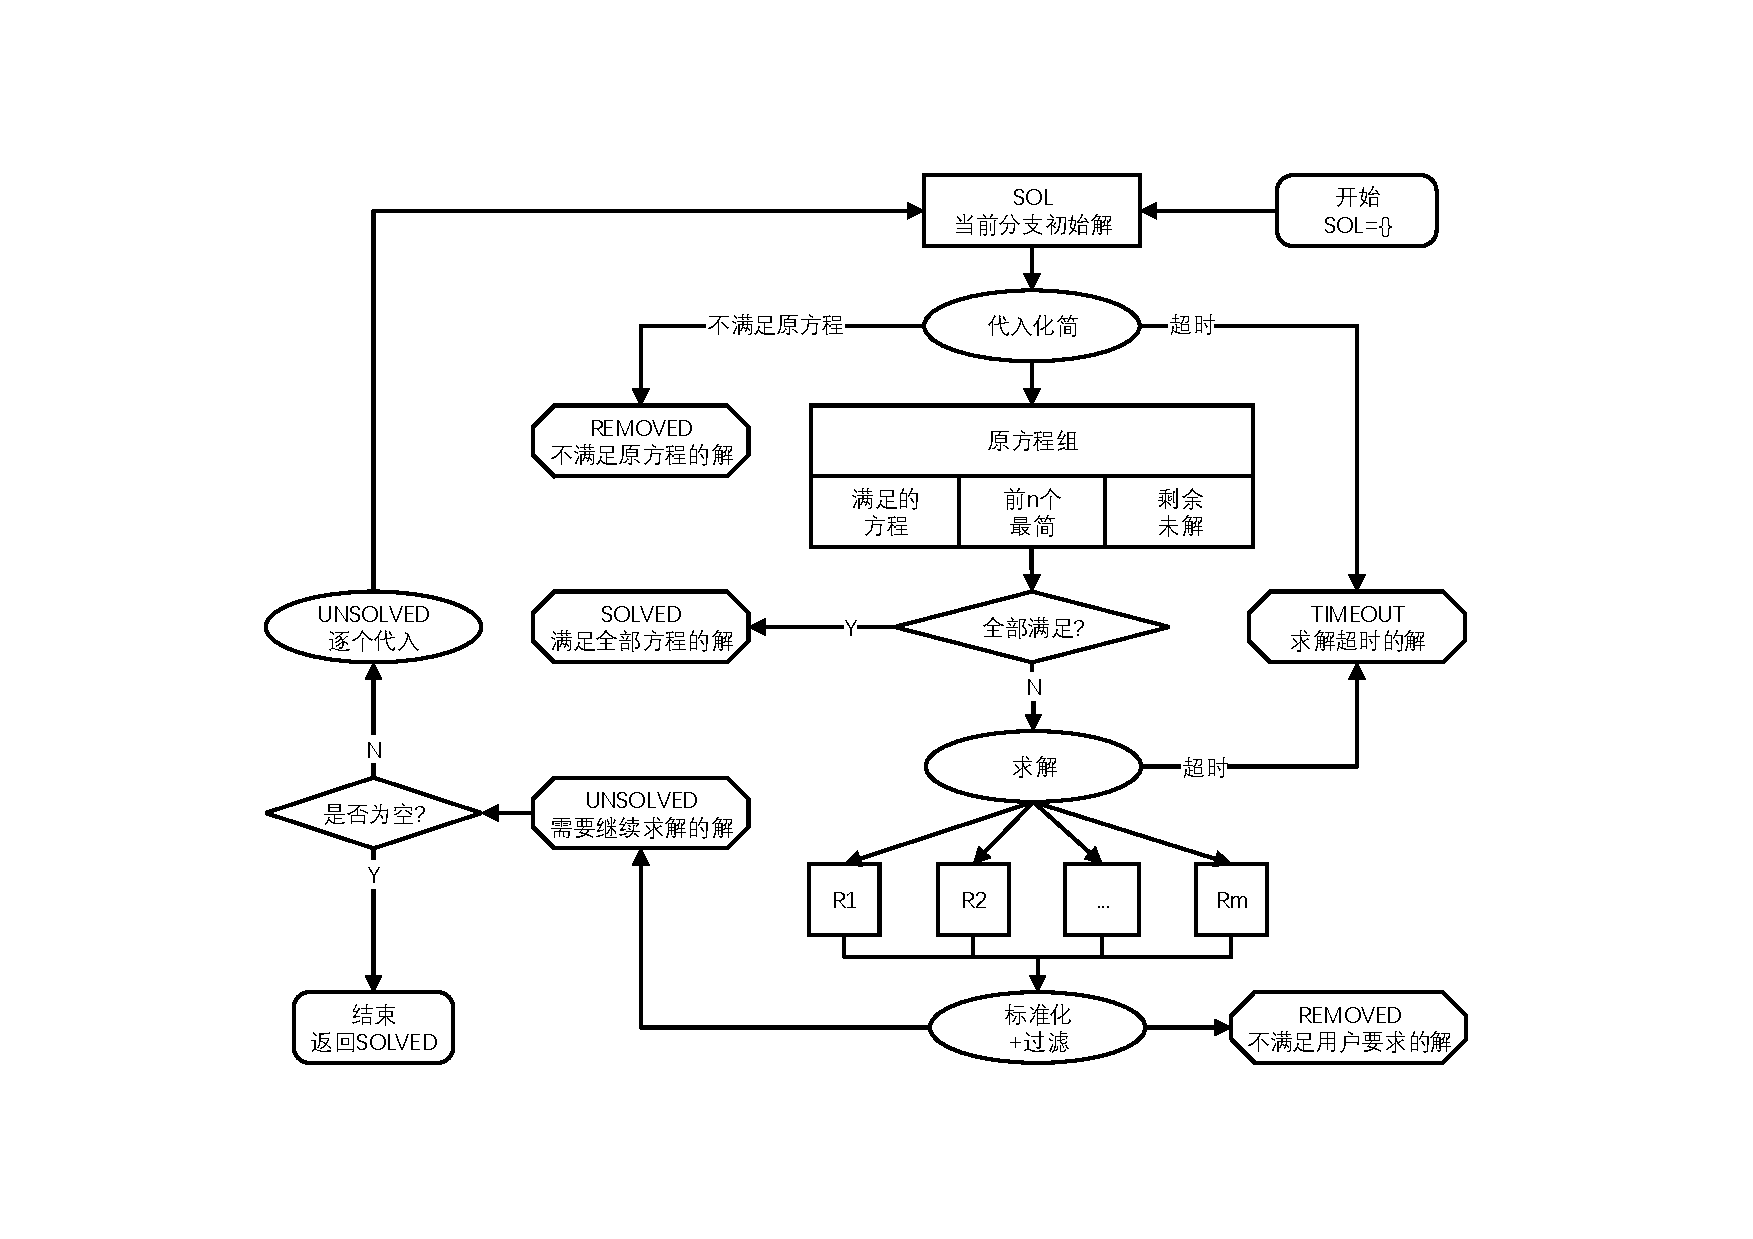
\includegraphics[height=0.8\textheight]{../paper/fig/pgsolve.pdf}
\end{figure}
\end{frame}

\begin{frame}
代入化简所有方程的优势:
\begin{enumerate}
\item 对尚未求解的方程进行代入化简, 能够对新的方程组按照复杂度重新排序, 从而获得更简单的方程.
\item 对已经求解过的方程进行代入化简, 能够验证当前分支的解是否满足这部分方程. 
\item 虽然单个分组只求解了$n$个方程, 但是获得的解可能满足更多的方程, 代入后可以及时地减少待求解方程的数量. 
\end{enumerate}
\end{frame}

\subsection{NS1L: 求n孤子-1 lump相互作用解的软件包}
\begin{frame}
\frametitle{NS1L: 求n孤子-1 lump相互作用解的软件包}
生成公式:
\[
    f_n=\sbrace{\xi_1+\eta_1}^2+\sbrace{\xi_2+\eta_2}^2+\sum_{i=1}^{2^n}\sbrace {q_i\prod_{k \in T_i}{\exp(\xi_{k+2})}}
\]
\[
    \xi_k=\sum_{j=1}^m{p_{j,k}x_j}
\]
约束条件:
\[
\begin{split}
    S&=\bbrace{\bbrace{q_i=0}|1\le i \le 2^n} \\ 
        &\cup \bbrace{\bbrace{p_{1,k}=0,\cdots,p_{m,k}=0}|1\le k \le n+2}  \\
        &\cup \bbrace{\bbrace{p_{j,1}=0,p_{j,2}=0}|1\le j \le m} \\ 
        &\cup \bbrace{\bbrace{p_{j,3}=0,\cdots,p_{j,n+2}=0}|1\le j \le m} . 
\end{split}
\]
对于一个解$t$ (是一个集合), 若存在$s\in S$, 满足$s\subseteq t$, 则$t$就不是我们想要的解.
\end{frame}

\begin{frame}
(3+1)YTSF 方程
\begin{figure}
\centering
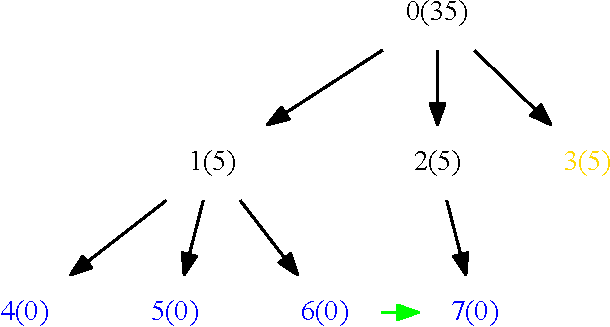
\includegraphics[width=.5\textwidth]{../paper/fig/0S1L.pdf}
\caption{0S-1L 求解分支图 (1秒)}
\end{figure}
\end{frame}

\begin{frame}
\begin{figure}
\centering
\setcounter{subfigure}{0}
\subfigure[]{
    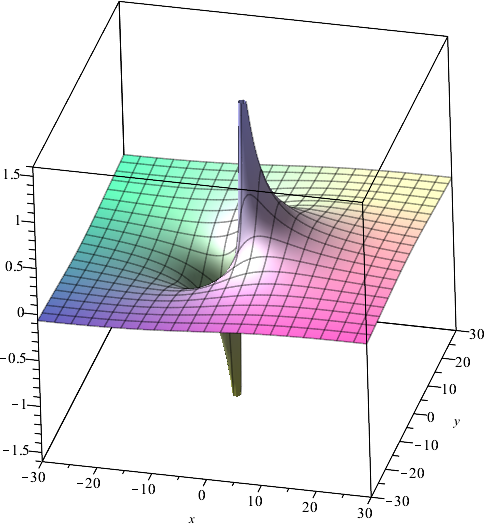
\includegraphics[width=.3\textwidth]{../paper/fig/0S1L-1.png}
}
\subfigure[]{
    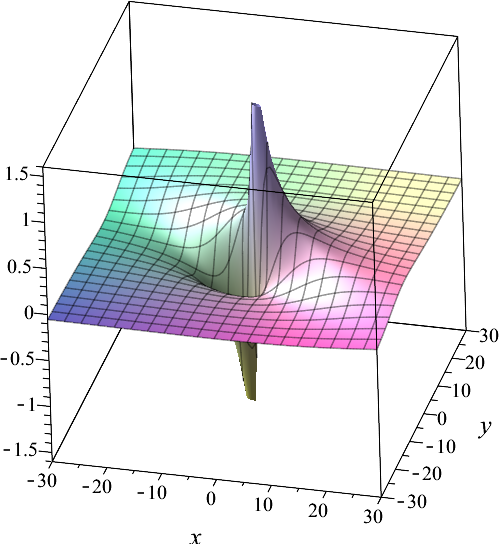
\includegraphics[width=.3\textwidth]{../paper/fig/0S1L-2.png}
}
\caption{(3+1)维 YTSF 方程的 0S-1L 解}
\end{figure}
\end{frame}


\begin{frame}
\begin{figure}
\centering
\setcounter{subfigure}{0}
\subfigure[1S-1L直接求解(8秒)]{
    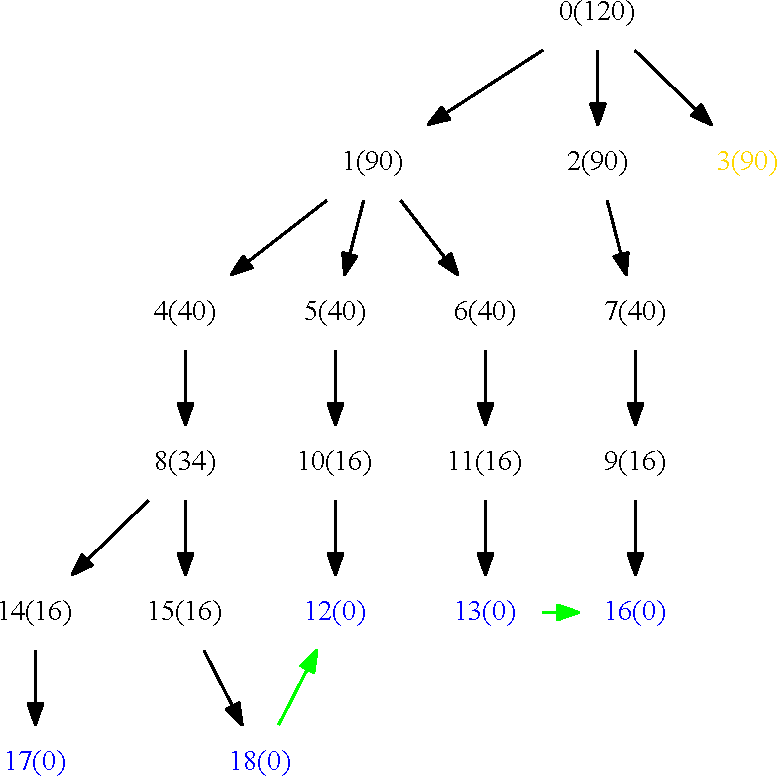
\includegraphics[width=.4\textwidth]{../paper/fig/1S1L-dir.pdf}
}
\hspace{2cm}
\subfigure[1S-1L继承求解(5秒)]{
    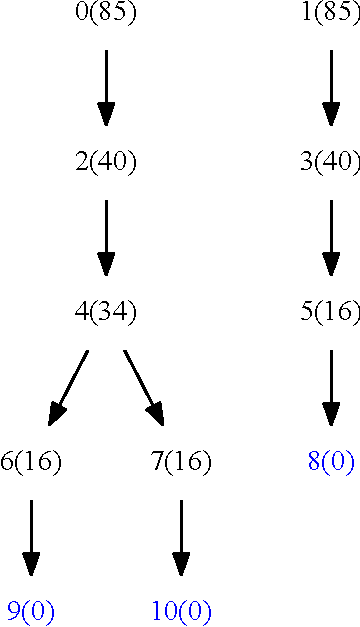
\includegraphics[width=.28\textwidth]{../paper/fig/1S1L-ext.pdf}
}
\end{figure}
\end{frame}

\begin{frame}
\begin{figure}
\centering
\setcounter{subfigure}{0}
\subfigure[]{
    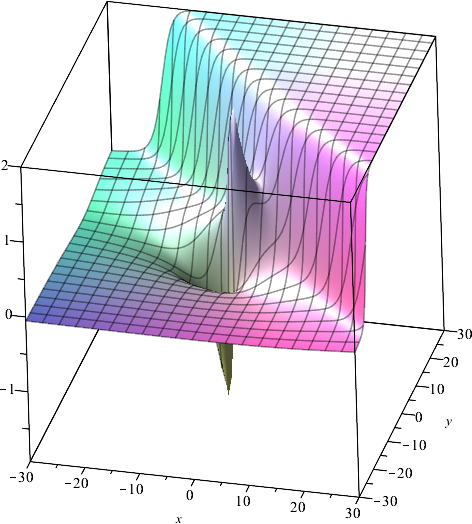
\includegraphics[width=.3\textwidth]{../paper/fig/1S1L-1.png}
}
\subfigure[]{
    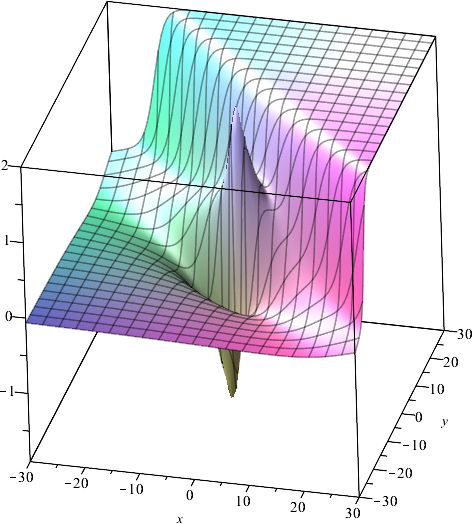
\includegraphics[width=.3\textwidth]{../paper/fig/1S1L-2.png}
}
\subfigure[]{
    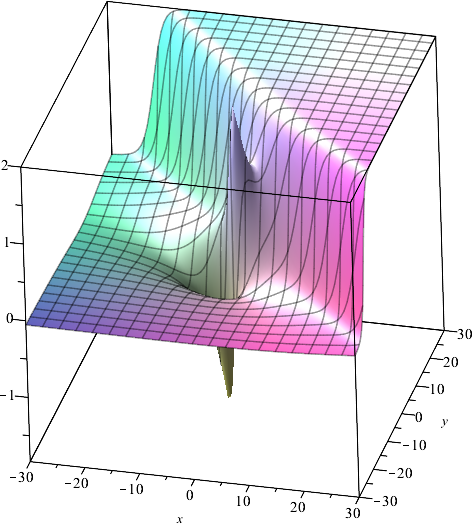
\includegraphics[width=.3\textwidth]{../paper/fig/1S1L-3.png}
}
\caption{(3+1)维 YTSF 方程的 1S-1L 解} \label{fig-1S1L}
\end{figure}
\end{frame}

\frame{
\begin{figure}
\centering
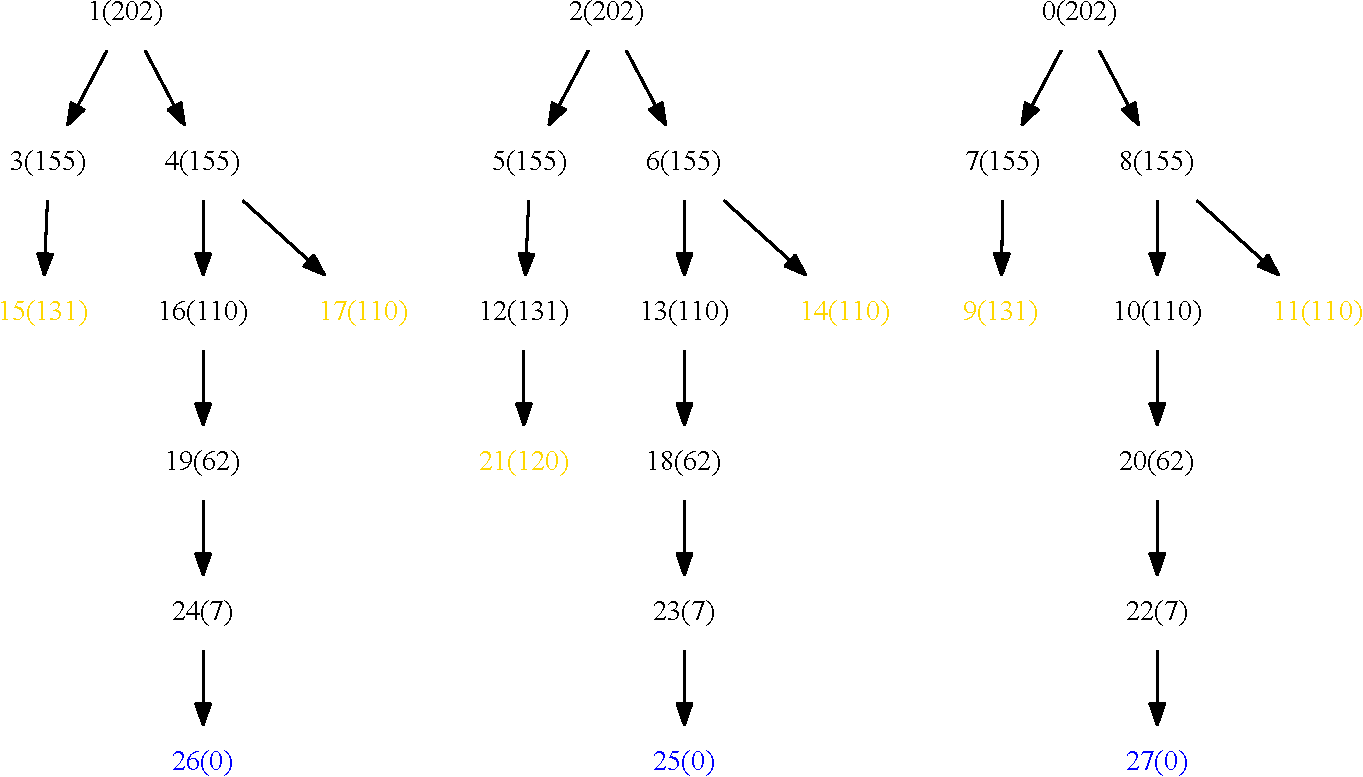
\includegraphics[width=\textwidth]{../paper/fig/2S1L-ext.pdf}
\caption{2S-1L 继承求解的分支图(30 秒)}\label{sb2-e}
\end{figure}
}

\frame{
\begin{figure}
\centering
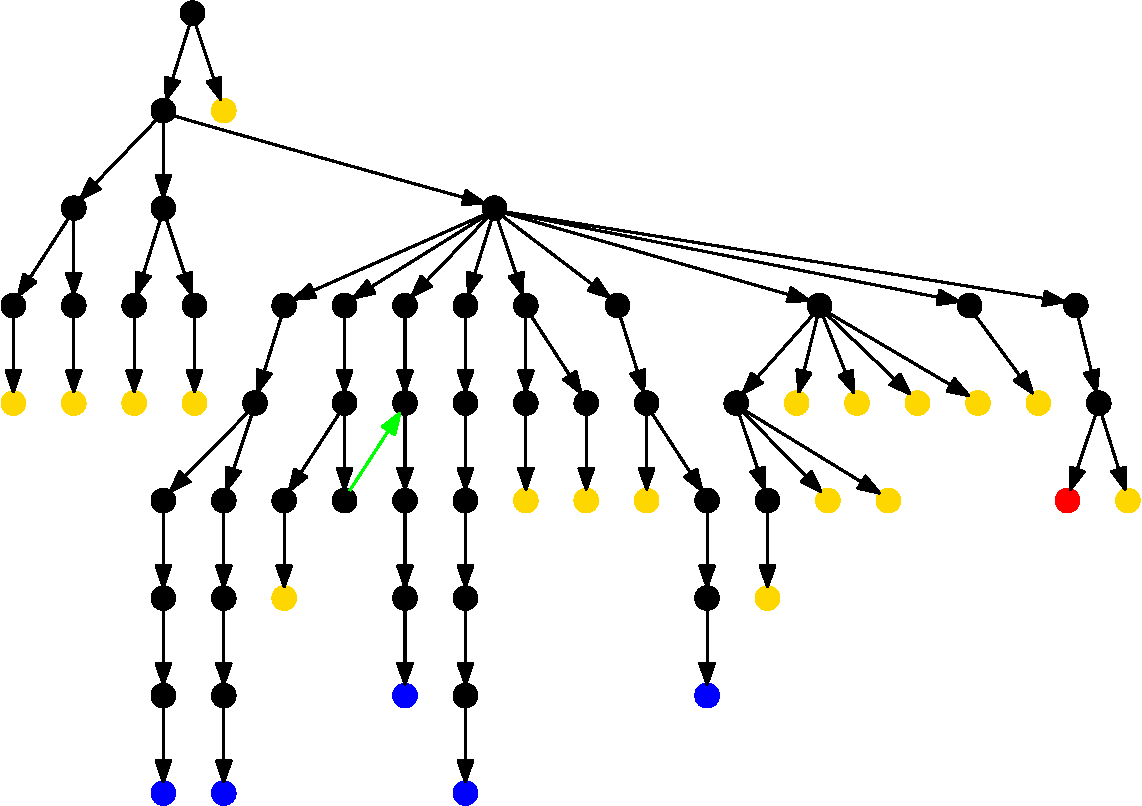
\includegraphics[height=0.8\textheight]{../paper/fig/2S1L-dir-point.pdf}
\caption{2S-1L 直接求解的分支图(430 秒)}\label{sb2-d}
\end{figure}
}

\frame{
\begin{figure}
\centering
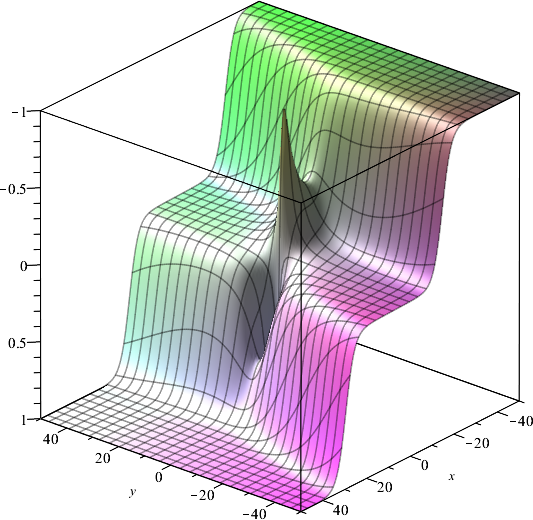
\includegraphics[width=.6\textwidth]{../paper/fig/2S1L.png}
\caption{(3+1)维 YTSF 方程的 2S-1L 解} \label{fig-2S1L}
\end{figure}
}

\subsection{PGSolve 的求解效率}
\begin{frame}
\frametitle{PGSolve 的求解效率}
\begin{adjustbox}{max width=\textwidth}
\centering
\renewcommand{\arraystretch}{1.3}
\begin{tabular}{cccccc}
\hline
来源方程 & 阶数 & 方程数 & 变量数 & PGSolve用时 & Solve用时 \\
\hline
(2+1) SK & 0 & 20 & 9 & 0.724 & 3.483 \\
(2+1) BKP-T & 0 & 20 & 9 & 0.571 & 3.486 \\
(2+1) KP & 0 & 35 & 9 & 1.759 & 29.643 \\
(3+1) YTSF & 0 & 35 & 11 & 1.229 & 8.839 \\
(3+1) JM & 0 & 35 & 11 & 0.845 & >1800 \\
(2+1) SK & 1 & 65 & 13 & 10.241 & >1800 \\
(3+1) YTSF & 1 & 120 & 16 & 12.228 & 1696.852 \\
\hline
\end{tabular}
\end{adjustbox}

\vspace{1em}

此处对比的是\cd{PDEtools:-Solve}. 而最常用的\cd{solve}函数甚至不能在 72 小时内求解只有 20 个方程的方程组, 这显然是\cd{solve}函数的一个 BUG.

\end{frame}

\begin{frame}

\begin{adjustbox}{max width=\textwidth}
\renewcommand{\arraystretch}{1.3}
\begin{tabular}{cccccc}
\hline
方程名称    & 解的阶数 & 方程数量 & 分组大小 & 解的个数 & 运行时间(s) \\ 
\hline 
(2+1)SK & 0 & 20 & 5 & 1 & 2.197 \\
(2+1)SK & 1 & 65 & 3 & 1 & 3.072 \\
(2+1)SK & 2 & 179 & 5 & 2 & 12.697 \\
(2+1)BKP-T & 0 & 20 & 5 & 1 & 1.036 \\
(2+1)BKP-T & 1 & 65 & 3 & 1 & 3.251 \\
(2+1)BKP-T & 2 & 179 & 5 & 2 & 12.617 \\
(3+1)YTSF & 0 & 35 & 5 & 2 & 1.948 \\
(3+1)YTSF & 1 & 120 & 5 & 3 & 6.717 \\
(3+1)YTSF & 2 & 324 & 5 & 3 & 37.909 \\
(3+1)JM & 0 & 35 & 5 & 3 & 2.014 \\
(3+1)JM & 1 & 120 & 5 & 13 & 18.384 \\
(3+1)JM & 2 & 324 & 5 & 4 & 50.934 \\
\hline 
\end{tabular}
\end{adjustbox}

\end{frame}

\subsection{软件展示}
\begin{frame}{软件展示}
\href{run:D:/Desktop/YjtMapleLib/build/LypReport/NS1L.mw}{NS1L.mw}
\begin{itemize}
\item 0S-1L 直接求解 
\item 1S-1L 直接求解和继承求解的对比
\item 2S-1L 继承求解
\end{itemize}
\end{frame}

\section{致谢}
\begin{frame}
\tikz[overlay,remember picture]\node[opacity=0.2]at (current page.center){
\includegraphics[width=0.7\paperheight]{../paper/sty/ecnu_logo.pdf}};
\centerline{\Huge 谢谢}
\end{frame}
\end{document}